\chapter{Theoretische Grundlagen}
\label{chap:theorie}
\qq{Warum NN?}
Künstliche Neuronale Netzwerke (kurz NN) dominieren den Forschungsbereich der 
Bilderkennung. 
Besonders die Klasse der faltenden Neuronalen Netzwerks \engl{convolutional neural network}, kurz CNN, konnte viele Erfolge für sich beanspruchen.
Rekordbrechende Ergebnisse bei der Klassifizierung von handgeschriebenen Ziffern \parencite{LeCunBackpropagationappliedhandwritten1989} und des ImageNet-Wettbewerbs \parencite{KrizhevskyImageNetClassificationDeep2012} motivieren dazu CNN-Methoden auch in anderen
Bereichen anzuwenden.

\mfigure{Diziplinen im Bereich Neuronale Netzwerke}{figures/theorie/nn_areas_venn.pdf}{fig:chen:cnn_task}

Neuronale Netzwerke benötigen weniger Entwicklungsaufwand und können zudem einfacher von 
 wachsenden Rechenkapazitäten und Datenmengen gebrauch machen \parencite[436]{LeCunDeeplearning2015}. 
Aber die Wissenschaft der NN ist ein Feld, dass durch die aktuelle Praxis mehr als durch Theorie geprägt ist. 
Das bedeuted zum einen das theoretische Grundlagen noch nicht gefestigt sind.
Zum anderen ist die Theorie nur eine Faktor für den erfolgreichen Einsatz von NNs. 
Je mehr Parameter unklar sind desto schwieriger wird eine Reproduktion.
\qq{Unterschied replikation, reproduktion?}
Die Reproduktion von Ergebnissen ist aber ein wichtiger Bestandteil in jedem Forschungsgebiet. 

\section{Maschinelles Lernen}
Neuronale Netzwerke und CNN sind Beispiele für Maschinenlernalgorithmen \engl{maschine learning algorithms}.
\cite{MitchellMachinelearning1997} definiert einen Maschinenlernalgorithmus wie folgt: ``A computer program is said to learn from experience E with respect to some class of tasks T and perfomance measure P, if its performance at tasks T, as measured by P improves with experience E''.

% experience E 
Die Erfahrung E kann zum Beispiel ein Datensatz \(X\) mit zugehörigen Klassen
\(Y\) sein. 
Im Fall der Dokumentensegmentierung kann ein Element \(x_i\) ein Bildauschnitt sein, 
dessen Kategorisierung ist dann das Label \(y_i\)(siehe \cref{fig:chen:cnn_task}).




% Task T 
Die Aufgabe T ist in den meisten Fällen eine statistische Modellierung.
Es wird angenommen, dass \(X\) und gegebenfalls \(Y\) mithilfe einer Wahrscheinlichkeitsfunktion \(p\)
modeliert werden können. 
Ein unüberwachter Lernalgorithmus versucht die Verteilung \(p(x)\) direkt zu lernen.
Beispiele für unüberwachte Algorithmen sind der k-Means-Algorithmus oder der PCA-Algorithmus.

Bei überwachten Lernalgorithmen wird versucht die Wahrscheinlichkeitsverteilung \(p(y | x)\) implizit zu ``lernen''.
Der Lernalgorithmus soll dabei eine Funktion finden \(f: \mathds{R}^n \rightarrow \left\{1,\dots,k \right\} \) so das \(y = f\left(x\right)\) \parencite[97 ff]{GoodfellowDeeplearning2016}.
Ein Lernalgorithmus der diese Funktion findet ist ein überwachter Lernalgorithmus \engl{supervised learning algorithm}
Die Trennung zwischen überwacht und unüberwacht ist nur eine grobe Einteilung. 
Tatsächlich sind die Übergänge fließend. 
Manche Maschinenlernverfahren benutzen beide Methoden.  

% perfrmance P
Die Performanz P der Vorhersagefunktion \(f\) wird im einfachsten Fall mit der Genauigkeit,
dem Verhähltniss von richtigen Vorhersage zu Falschen, gemessen. 
% TODO: Tabelle
\cref{tab:truth}
\begin{table}
    \caption{Wahrheitstabelle}
    \label{tab:truth}
    \begin{tabular}{llll}
                    &&\(y\)& \\
                            && Positiv       & Negativ \\
    \(\hat{y}\) & Positiv  & true positive  & false positive \\
                & Negativ & false negatve   & true negatve \\
    \end{tabular}       
\end{table}    
\section{Künstliche Neuronale Netzwerke}

Künstliche Neuronale Netzwerke \kurz{KNN} sind eine Modellierungsmethode des statistischen Lernens, die von der Natur inspiriert wurde. 
Das Neuron ist der Grundbaustein eines Netzwerkes und verarbeitet eingehende Signale. 
Ein KNN besteht meistens aus zwei Teilen: einer linearen Funktion über die Eingabesignale und 
einer nicht-linearen Aktivierungsfunktion.

Zur besseren Erläuterung der Theorie soll hier ein Teilproblem der Dokumentensegmentierung dienen.
In diesem Fall besteht der Datensatz \(X\) aus Bildausschnitten die im Bildzentrum Text enthalten.
Wenn ein Element \(x_i\) Text enthählt, dann ist das \(y_i = 1\) andernfalls \(0\).

\sfigure{Bildauschnitte mit und ohne Textinhalt}{figures/chen/cnn_task.pdf}%{fig:chen:cnn_task}

\begin{align}
    f \left(\raisebox{-.5\height}{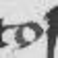
\includegraphics{figures/chen/text_tile.pdf}}\right) = 1
\end{align}

Wir wollen eine Funktion finden, die mit hoher Wahrscheinlichkeit eine Vorhersage 

\begin{align}
    \theta_{ML} = \argmax_{\theta} P(Y | X, \theta)
\end{align}

Das einfachste Beispiel ist die Klasse der vollvernetzen KNN. 
Jedes Element in einem Eingangssignalvektor \(x\) wird mit einem Parameter aus dem Gewichtsvektor \(w\) verechnet. Dazu kommt der Biaswert \(b\).

\begin{align}
    \hat { y } = w^{ \top } x + b
\end{align}



\begin{align}
    f(X)=\sum\limits_{m=1}^{M}g_{m}\left(\omega_{m}^{\top}X\right)
   \end{align}
Target als nonlineare Funktion dieser Features modelieren.  



\section{Aktivierungsfunktionen}
\begin{align}
    \operatorname{softmax}(z)_{i}=\frac{\exp\left(z_{i}\right)}{ \sum _ { j } \exp \left( z _ { j } \right) }
\end{align}
% TODO: set font size??? 
\begin{figure}
    \caption{ReLU- und Sigmoid-Funktionsplot}
    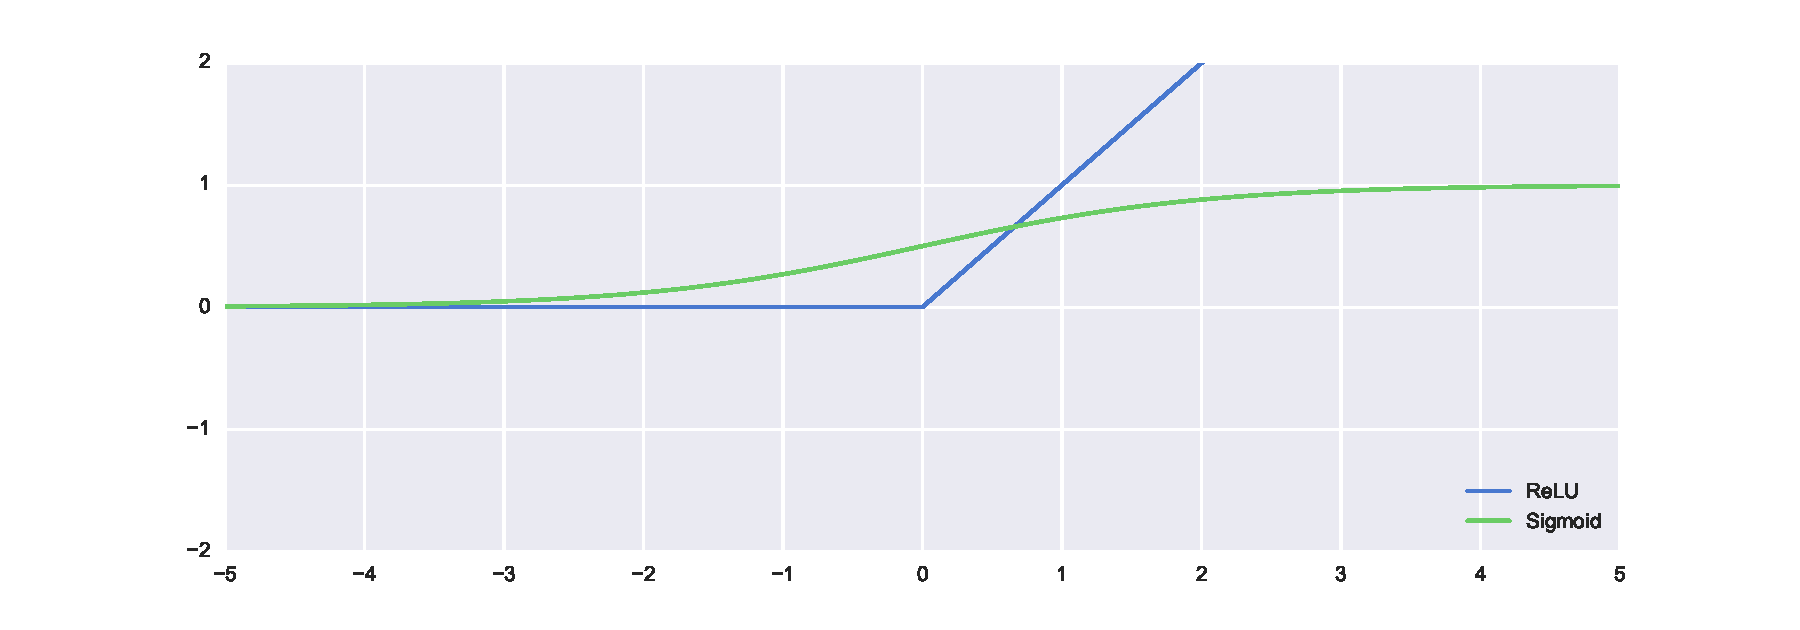
\includegraphics[width=\textwidth]{figures/plot/relu_sigmoid.pdf}
\end{figure}

\subsection{ReLU}
\begin{align}
    f\left(x\right) &= \text{max}(0,x)
\end{align}
\subsection{Softmax}


\section{SGD}
\section{Xavier initialization}
\section{Regularisierung}
\label{sec:Regularisierung}
Durch SGD und in kleinen Datensets ensteht Samplingrauschen \engl{sampling noise}. 
Eine kleine Auswahl von Beispielen kann Zusammenhänge enthalten, 
die nicht in der tatsächlichen Verteilung der Daten vorhanden ist.
Regularisierung können helfen eine Überanpassung des Models zu verhindern.
\subsection{Dropout}

Dropout ist eine Regularisierungsmethode für Neuronale Netzwerke, 
die versucht durch zufälliges Ausschalten einzelner Aktivierungen koadaptionen zu verhindern.

Während einer Trainingsiteration wird ein Element mit einer Wahrscheinlichkeit \(p\) ausgeschaltet (Aktivierung gleich 0).
Dadurch wird bei jedem Trainingsschritt ein anderes Modell trainiert. 
In der Testphase werden die Gewichte mit \(p\) skaliert. 

Netzwerke mit Dropout generalisieren besser auf noch nicht gesehene Daten.
\subsection{Weight decay}


\section{CNN}
\qq{Nachtteile fully connected NN für Bilderverarbeitung}
Die Anzahl der Parameter in der Gewichtsmatrix \(W\) wird von der Größe des Inputs bestimmt.
Möchte man Bilder ein Bild mit der der 

\qq{Sind Filter vorläufer von CNN?}
CNN kombinieren zwei Konzepte der Bilderverarbeitung: Neuronale Netzwerke und Filter.
Klassifikationsprobleme wurde traditionell in zwei Schritten gelöst. Zuerst wurden 
Featuredeskriptoren entwickelt welche dann als Input für trainierbare Klassifizierer 
verwendet wurden \autocite[2353]{RawatDeepConvolutionalNeural2017}.


\qq{Was ist convolutional?}
So können zum Beipspiel Kanten in einem Bild ein Klassifizerungsgrundbaustein sein. 
Um die Kanten in einem Bild zu finden wird das Bild mit einem Kernel  gefaltet.  
Der Begriff Faltung wird üblicherweise für die Verknüpfung von zwei realwertigen Funktione verwendet. Die analoge Form der Faltung ist eine lineare , translations-invariante Funktion, siehe \cite[28]{SusseBildverarbeitungundObjekterkennung2014}. 
\begin{align}
    \label{eq:convolutional}
    convolutional
\end{align}
Im Bereich der Bilderverarbeitung wird schon länger eine abgeänderte Faltungsfunktion genutzt: die Autokorrelation \engl{cross-correlation}. Bild und Filter sind 2D-Funktionen die zum einen nur für diskrete Intervale definiert sind zum anderen für Bereiche aushalb des ihres Definitionsbereichs gleich 0 sind. Zudem wird überlicherweise der Index für den Kernel addiert (siehe \cref{eq:convolutional}).
\begin{align}
    \label{eq:crosscorrelation}
    I*K(i,j) =
\end{align}


Ein CNN ist eine Neuronales Netzwerk, dass in mindesten einen Layer die Faltung anstatt der normalen Matrixmultiplikation verwendet \parencite[321]{GoodfellowDeeplearning2016}.
\qq{Drei Hauptvorteile?}
\cite{GoodfellowDeeplearning2016} sieht drei Vorteile von CNN gegenüber voll-vernetzten NN: verringerte Konnektivität, 
gemeinsame Parameternutzung, eqivariante Darstellung.
Wie schon erwähnt steigt die Anzahl der Parameter in einem voll-vernetzten NN je größer der Input wird, weil jedes Neuron mit jeder Aktivierung der vorhergehenden Schicht verbunden ist. 
Durch die Faltungsoperation erhählt jedes Neuron nur die Signale die im Bereich des Filterkernels liegen. Dieser Bereich wird auch rezeptives Feld genannnt.
Durch die Schichtung von mehreren Faltungen vergrößert sich das rezeptive Feld der Neuronen in tieferen Schichten (siehe \cref{fig:cnn_neurons}).


\begin{marginfigure}
    \label{fig:cnn_neurons}
    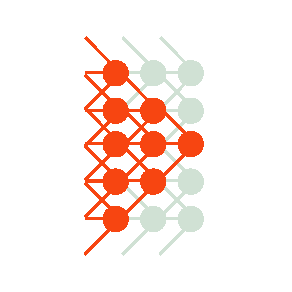
\includegraphics[width=\textwidth]{figures/theorie/perceptive_field.pdf}
    \caption{Rezeptives Feld in einem mehrschichtigen Netz}
\end{marginfigure}

\qq{Nachteile CNN?}
\qq{Filterbeispiel?}
\qq{}


\section{Vorverarbeitung}
Für die Verarbeitung von Dokumentenseiten werden meistens noch weitere Algorithmen eingesetz um Klassifizierung und Segmentierung zu erleichtern. 
Da wir nur an Inhalten interessiert sind die auf ein Medium aufgetragen wurden (z.B. Tinte auf Papier) ist eine Binarisierung des Bildes ein hilfreicher Schritt. 
Eine Binarisierungsfunktion soll Werte der bildgebenden Funktion auf zwei Werte, 
jeweils für Vorder- und Hintergrund, abbilden
\(bin(I): f: i \in \left\{0 \dots 255\right\} \rightarrow b \in \right\{0, 1\right\} \)

Dokumentenbilder haben zudem oft eine sehr hohe Auflösung und enthalten Prozentual nur wenig Vordergrundpixel.

\section{SLIC Superpixel}
Der SLIC-Algorithmus basiert auf dem k-Means-Algorithmus und teilt Pixel inhalb eines 5D-Raums in Cluster ein. 
In jedem Arbeitsschritt werden Pixel dem Clusterzentrum mit der geringsten Distanz zugeordnet und danach werden die Clusterzentren neu berechnet.
Das Distanzmaß \(D_s\) zu den Clusterzentren \(k=[1,K]\) basiert auf den Farbabstand im Lab-Farbraum \(d_{lab}\) und den räumlichen Abstand \(d_{xy}\):

\begin{align}
    d_{lab} &= \sqrt{ \left( l_k - l_i \right)^2 + \left( a_k - a_i \right)^2 + \left( b_k - b_i \right)^2 }\\
    d_{xy}  &= \sqrt{ \left( x_k - x_i \right)^2 + \left(y_k - y_i \right)^2 }\\
    D_{s}   &= d_{lab} + \frac{m}{S} d_{xy}
\end{align}

Der Faktor \(m\) ermöglicht eine Gewichtung der zwei Distanzmaße. 
Je höher der Faktor desto kompakter werden die Superpixel. \cref{fig:slic_parameters}
zeigt das Ergebniss des Algorithmus mit unterschiedlichen Parameter  \(m\)
angewendet auf eine Dokumentenseite.
